\section{Rich Picture Overview??}
This section will provide an overview of the chosen solution using rich pictures.

The server-station relationship is shown in \figref{fig:ServerRichPicture}. 
The server contains collected information from each station, such as bookings, amount of available bicycles at stations, and usage statistics.
It provides booking and amount of available bicycles at stations through a webpage to the user. 
Usage statistics are provided to the facilitators of the system and gives them the ability to improve it. 

\begin{figure}[h]
\centering
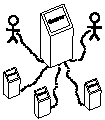
\includegraphics[scale=3]{serverrichpicture/server.pdf}
\caption{The server and the associated stations.}
\label{fig:ServerRichPicture}
\end{figure}

The stations receive the information that allows it to handle bookings done on the server.
They also have the capability of handling booking by themselves, which is then shared with the central server.
Sharing information such as the amount of available bicycles is also something the stations need to be able to do.
The dock that provide the locking/unlocking mechanism along with the bicycle detection ability have to talk to the station, for example when they need to unlock booked bicycle this information needs to be propagated from the server to the station to the individual bicycle.
This can be seen in \figref{fig:StationRichPicture}.

\begin{figure}[h]
\centering
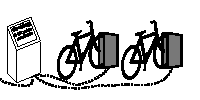
\includegraphics[scale=3]{stationrichpicture/station.pdf}
\caption{The station and the bikes.}
\label{fig:StationRichPicture}
\end{figure}

\begin{comment}
\begin{figure}[h]
\centering
\begin{subfigure}[b]{0.3\textwidth}
\centering

\includegraphics[scale=1]{Bicyclewithlock/bicylewithlock.pdf}
\caption{Locked bicycle.}
\label{fig:BicycleLocked}
\end{subfigure}
~
\begin{subfigure}[b]{0.3\textwidth}
\centering

\includegraphics[scale=1]{Bicyclewithoutlock/bicylewithoutlock.pdf}
\caption{Unlocked bicycle.}
\label{fig:BicycleUnlocked}
\end{subfigure}
\caption{Rich picture of bicycle.}
\label{fig:Bicycles}
\end{figure}
\end{comment}